%!TEX root = masters-dissertation.tex
\chapter{Background}
\label{chapter:background}



\section{Environments}
\label{sec:environments}

In the context of multi-agent systems, the environment is the world in which agents act.
The design of an agent-based system must take into consideration the environment in which the agents are expected to act, since it determines which AI techniques are needed for the resulting agents to accomplish their design goals. 
Environments are often classified according to the following attributes~\cite{russell1995artificial}:  observability, determinism, dynamicity, discreteness, and the number of agents. 

The first way to classify an environment is related to its observability. 
An environment can be unobservable, partially observable, or fully observable. 
For example, the real world is partially observable, since each person can only perceive what is around his or herself, and usually only artificial environments are fully observable.
% 
The second way to classify an environment, is about its determinism.
In general, an environment can be classified as stochastic or deterministic.
In deterministic environments, an agent that performs an action $a$ in a state $s$ always result in a transition to the same state $s'$, no matter how many times the process is repeated, whereas in stochastic environments there can be multiple possible resulting states $s'$, each of which has a specific transition probability.
% 
The third way to classify an environment is about its dynamics. 
Static environments do not change their transition dynamics over time, while dynamic environments may change their transition function over time. 
% 
Moreover an environment can be classified as continuous or discrete.
Discrete environments have a countable number of possible states, while continuous environments have an infinite number of states.
A good example of discrete environment is a chessboard, while a good example of continuous environment is a real-world football pitch. 
% 
Finally, environments are classified by the number of agents acting concurrently, as either single-agent or multi-agent. 
In single-agent environments, the agent operates by itself in the system (no other agent modifies the environment concurrently) while in multi-agent environments agents can act simultaneously, competing or cooperating with each other. 
A crossword game is a single-agent environment whereas a chess game is a multi-agent environment, where  two agents take turns acting in a competitive setting.



\section{Markov Decision Process}
\label{sec:markov}

Agents need to make careful decisions, since today's decisions can impact on tomorrow's and tomorrow's on the next day.
Markov Decision Process (MDP), also known as stochastic control problems~\cite{puterman1994markov}, is a model used to represent sequential decision making when its consequences are not deterministic.
That is, MDP is a mathematical model used for modeling decision making where choices of actions are partly random and partly under the control of an agent.
An MDP is represented by a tuple $\langle S, A, T, R\rangle$~\cite{graepel2004learningfight, taylor2011teachingmario} consisting of

1. a \textit{state space S} is a finite set of states $s \in S$.
You could say that the state space is a set of bindings of values to variables.
In computer games, one state represents a set of characteristics about the game, such as:
the character is on the ground, is jumping, is facing a wall, is carrying certain items, the current life (health bar) from the character, etc.;

2. a \textit{action space A} with a finite set of actions $a \in A$.
Actions are responsible for change the game states. In computer games, action could be things like:
jump, shoot, move left, move forward, pick up an item, etc..;

3. A \textit{transition probabilities T} represents a set of probabilities of transitions given by
$T : S \times A \mapsto S$. The probability function is generally defined as:
$P(s' \mid s,a)$ and represents the transition probability of a state $s$ to $s'$ when
an action is performed by the agent;

4. a \textit{reward function} $R : S \times A \times S' \mapsto \mathbb{R}$.
The reward is one of the key elements in the learning process, since it describes
the \textit{feedback} the agent use to improve himself.
In fighting games~\cite{graepel2004learningfight}, for example, the reward could be given
by the difference from the values of the life bar between both characters, after an action is performed;

Figure~\ref{fig:mdp} represents a MDP with three states ($S_0$, $S_1$ and $S_2$) and
two actions ($a_0$ and $a_1$). In this example, each state has two avaliable actions,
each of these actions lead to a new state. An action can lead to different states with different probabilities.
For example: at state $S_2$, if the action $a_0$ is executed, there is 40\% (0.4) chance to
reaching the state $S_0$ and 60\% (0.6) chance of remaining at the same state ($S_2$).
After the state transition occurs through the execution of an action, the agent receives feedback that can be
either positive or negative --- in Figure~\ref{fig:mdp} feedback from performing action $a_0$ at state $S_1$
and reaching state $S_0$ is $+5$, while performing the action $a_1$ at state $S_2$ and reaching state $S_0$
is $-1$.

\begin{figure}
\centering
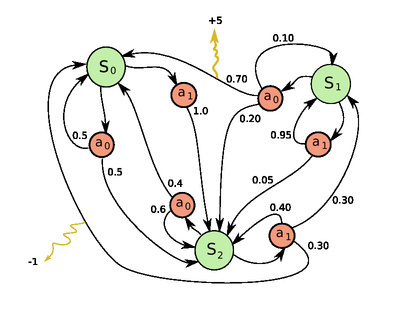
\includegraphics[width=300px]{images/mdp}
\caption{An example of MDP with three states and two actions.}
\label{fig:mdp}
\end{figure}

An MDP is a mapping from states to actions that tells an agent what to do at each state~\cite{bellman1957dynamic,dreyfus2002richard}.
MDPs can be used to find optimal policies --- i.e., a kind a mapping of each state to the action that yields the highest long-term reward.
An optimal policy~\cite{morin1982monotonicity, mitten1964composition} is the policy that 
maximizes the reward obtained for each state/action~\cite{guelpeli2003utilizaccao}.
An optimal policy is a policy that, for each state, sets the action whose expected reward is maximized at infinite time.
The Bellman's Principle of Optimality states that 
all parts of an optimal solution must also be optimal~\cite{morin1982monotonicity}:
\textit{
``An optimal policy has the property that, whatever the state and the initial decision,
upcoming decisions from the resulting state must also be an optimal policy''}~\cite[p. 83]{bellman1957dynamic}.

The Bellman equation describes the optimal policy for an MDP whose parameters are known 
--- ie, all states, actions, and transitions probabilities are known and are represented by:
\[
	V(s) \leftarrow \left[max_a \gamma \sum_{s'}^n P(s'|s,a) * V(s')\right] + R(s)
\]
Where,
\begin{itemize}
\item $s$ represents a MDP's state;
\item $a$ represents an action, responsible for the transition between the states of the MDP;
\item $n$ represents the number of possible actions at the state $s$;
\item $s'$ represents the state resulting from the execution of the action $a$ at state $s$;
\item $V(s)$ is the long term value of $s$;
\item $R(s)$ is the immediate reward at state $s$;
\item $\gamma$ is the \textit{discount factor}, which determines the importance of future rewards --- a factor of $0$ makes the agent opportunistic~\cite{schweighofer2003meta} by considering only the current reward, while a factor of $1$ makes the agent consider future rewards, seeking to increase their long-term rewards;
\end{itemize}

$max_a \gamma \sum_{s'}^N P(s'|s,a) * V(s')$ represents the best action to perform at the state $s$.
It is part of the value iteration algorithm responsible for seeking the optimal action,
at the state with the highest obtainable value from the current state.



\section{Machine Learning}
\label{sec:machine-learning}

An agent is said to be learning if it improves its performance after observing the world around it~\cite{russell1995artificial}. 
Common issues in the use of learning in computer games include questions such as whether to use learning at all, or wether or not insert improvement directly into the agent code if it is possible to improve the performance of an agent. 
Russell and Norvig~\cite{russell1995artificial} state that it is not always possible or desirable, to directly code improvements into an agent's behavior for a number of reasons. First, in most environments, it is difficult to enumerate all situations an agent may find itself in. Furthermore, in dynamic environments, it is often impossible to predict all the changes over time. And finally, the programmer often has no idea of an algorithmic solution to the problem, so it is better to let a learning algorithm achieve the desired results.

Thus, in order to create computer programs that change behavior with experience, learning algorithms are employed. 
There are three main methods of learning, depending on the feedback available to the agent. 
In \emph{supervised learning}, the agent approximates a function of input/output from observed examples. 
In \emph{unsupervised learning}, the agent learns patterns of information without knowledge of the expected classification. 
In \emph{reinforcement learning}, the agent learns optimal behavior by acting on the environment and observing/experiencing rewards and punishments for its actions. 
In this work, we focus in reinforcement learning technique. 



\section{Reinforcement Learning}
\label{sec:rl}

When an agent carries out an unknown task for the first time, it does not know exactly whether it is making good or bad decisions. 
Over time, the agent makes a mixture of optimal, near optimal, or completely suboptimal decisions. 
By making these decisions and analyzing the results of each action, it can learn the best actions at each state in the environment, and eventually discover what the best action for each state is. 

Reinforcement learning (RL) is a learning technique for agents acting in a stochastic, dynamic and partially observable environments, observing the reached states and the received rewards at each step~\cite{sutton1998reinforcement}. 
Figure~\ref{fig:rl} illustrates the basic process of reinforcement learning, where the agent performs actions, and learns from their feedback. 
An RL agent is assumed to select actions following a mapping of each possible environment state to an action. 
This mapping of states to actions is called a \emph{policy}, and reinforcement learning algorithms aim to find the \emph{optimal policy} for an agent, that is, a policy that ensure long term optimal rewards for each state. 

\begin{figure}[ht]
\centering
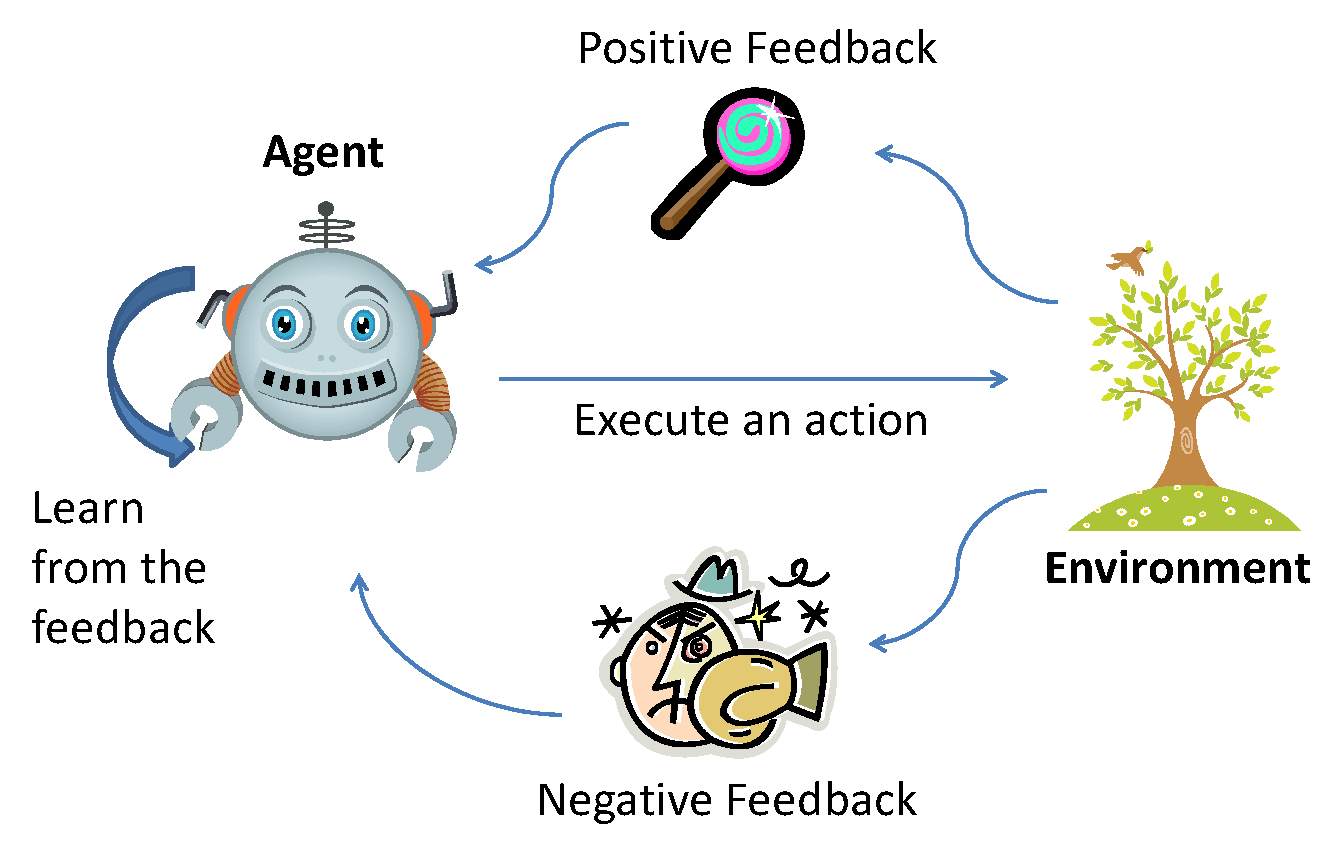
\includegraphics[width=400px]{images/rl}
\caption{Model to describe the process of reinforcement learning.}
\label{fig:rl}
\end{figure}

RL techniques are divided into two types, depending on whether the agent changes acts on the knowledge gained during policy execution~\cite{russell1995artificial}. 
In \emph{passive RL}, the agent simply executes a policy using the rewards obtained to update the \emph{value} (long term reward) of each state, whereas in \emph{active RL}, the agent uses the new values to change its policy after a certain number of iterations.
A passive agent has a fixed policy: at state $s$, the agent always performs the same action $a$.
Its mission is to learn how good its policy is --- to learn the utility of it.
An active agent has to decide what actions to take in each state:
it uses the information obtained by reinforcement learning to improve its policy. 
By changing its policy in response to learned values, an RL agent might start exploring different parts of the environment. 
Nevertheless, the initial policy still biases the agent to visit certain parts of the environment~\cite{russell1995artificial}, so an agent needs to have a policy to balance the use of recently acquired knowledge about visited states with the exploration of unknown states in order to approximate the optimal values~\cite{ghory2004boardgames}. 



\subsection{Q-Learning}
\label{subsec:ql}

Depending on the assumptions about the agent knowledge prior to learning, different algorithms can be used. 
When the rewards and the transitions are unknown, one of the most popular reinforcement learning techniques is \textit{Q-learning}. 
This method updates the value of a pair of state and action --- named state-action pair, $Q(s,a)$ ---
after each action performed using the immediately reward. 
When an action $a$ is taken at a state $s$, the value of state-action pair, or Q-value,
is updated using the following adjustment function~\cite{amato2010highlevel}.
% 
	$$Q(s,a) \leftarrow Q(s,a) + \alpha[r + \gamma max_{a' \in A(s')}Q(s',a') - Q(s,a)]$$
% 

Where, 
\begin{itemize}
\item $s$ represents the current state of the world;
\item $a$ represents the last action chosen by the agent;
\item $ Q(s,a) $ represents the value obtained the last time action $a$ was executed at state $s$.
This value is often called Q-value.
\item $r$ represents the reward obtained after performing action $a$ in state $s$;
\item $s'$ represents the state reached after performing action $a$ in state $s$;
\item $a' \in A(s')$ represents a possible action from state $s'$;
\item $max_{a' \in A(s')}Q(s',a')$ represents the maximum Q-value that can be obtained from the state $s'$, independently of the action chosen;
\item $\alpha$ is the learning-rate, which determines the weight of new information over what the agent already knows --- a factor of $0$ prevents the agent from learning anything (by keeping the Q-value identical to its previous value) whereas a factor of $1$ makes the agent consider all newly obtained information;
\item $\gamma$ is the same \textit{discount factor} as in~\ref{sec:markov};
\end{itemize}

Once the Q-values are computed, an agent can extract the best policy known so far ($\pi^{\approx}$) by selecting the actions that yield the highest expected rewards using the following rule:
$$\pi^{\approx}(s) = \arg\max_{a}Q(s,a) $$

The complete algorithm for an exploratory Q-learning agent is show in~\ref{alg:Qlearning}.

\begin{algorithm}
	\caption{An exploratory Q-learning agent that returns an action after receiving immediate feedback}
	\label{alg:Qlearning}
	\begin{algorithmic}[1]
		\REQUIRE $s, a, r$
		\IF{TERMINAL?(s)}
			\STATE $Q(s,None) \gets r$
			\STATE $a' \gets None$
		\ELSE
			\STATE $Q(s,a) \gets Q(s,a) + \alpha[r + \gamma max_{a' \in A(s')}Q(s',a') - Q(s,a)]$
			\STATE $a' \gets \pi^{\approx}(s)$
		\ENDIF
		\RETURN $a'$
	\end{algorithmic}
\end{algorithm}

Q-learning converges to an optimal policy after visiting each state-action pair a sufficient number of times, but it often requires many learning episodes~\cite{watkins1992technical}.
In dynamic environments, Q-learning does not guarantee convergence to the optimal policy since it is possible that the required number of leaning episodes never occurs.
This occurs because the environment is always changing and demanding that the agent adapts to new transition and reward functions.
However, Q-learning has been proven efficient in stochastic environments 
even without convergence~\cite{sandholm1996multiagent,tesauro2002pricing,amato2010highlevel}.
In multi-agent systems where the learning agent models the behavior of all other agents as a stochastic environment (an MDP), Q-learning provides the optimal solution when these other agents
-- or players in the case of human agents in computer games --- do not change their policy choice. 



\subsection{Dyna-Q}
\label{subsec:dynaq}

Learning a model means to learn the transition probabilities, the reward values for each state and action, or both simultaneously.
It is possible to find optimal policies when the parameters model are known.
One can learn the parameters of a model through the simulation of a template --- this model can be evaluated by using passive reinforcement learning, as seen previously (Section~\ref{sec:rl}).
Dyna-Q~\cite{sutton1991dyna} is an approach which first builds a correct model, then find the policies through this model~\cite{kaelbling1996reinforcement}.
This approach first learns the parameters of a model and then uses this definition of parameters to calculate the optimal policy learned about the model~\cite{amato2010highlevel}.

Dyna-Q can use the model to generate learning experiences --- simulate the learning within a built model --- and learn the Q-values more quickly than simply applying Q-learning.
The agent learns both model and Q-values through executing its actions on environment.
The model is used to simulate the environment and update the Q-values.
The better the representation of model parameters, faster the convergence of learning will occur.
The algorithm Dyna-Q operates learning the model at each step, and then applying the technique of Q-learning to learn the model's policy.

\begin{algorithm}
	\caption{Dyna-Q}
	\label{alg:dynaQ}
	\begin{algorithmic}[1]
		\REQUIRE $Q, r, s, a, numIter$
		\item[]
		\STATE $Q(s,a) \gets Q(s,a) + \alpha(r + \gamma max_{a' \in A(s')}Q(s',a') - Q(s,a))$
		\STATE $P(s'|s,a) \gets updatePAverage(s,a,s')$
		\STATE $R(s,a) \gets updateRAverage(s,a)$
		\item[]
		\FOR{$i = 0$ \TO $numIter$}
        	\STATE $s' \gets randomPreviouslySeenS()$
        	\STATE $a' \gets randomPreviouslyTakenA(s')$
        	\STATE $s'' \gets sampleFromModel(s',a')$
        	\STATE $r' \gets fromModel(s',a')$
        	\STATE $Q(s,a) \leftarrow Q(s,a) + \alpha[r + \gamma max_{a' \in A(s')}Q(s',a') - Q(s,a)]$
		\ENDFOR
		\item[]
		\RETURN $Q$
	\end{algorithmic}
\end{algorithm}

Dyna-Q is shown in Algorithm~\ref{alg:dynaQ}. The first step of Dyna-Q is to update the value of $Q$ using Q-learning.
The transition probability ($updatePAverage$ function from the algorithm) is given by the number of times the agent has chosen action $a$ at state $s$ and reached state $s'$, divided by the number of times the agent was in state $s$ and chose the action $a$:
\[ P(s'|s,a) = \frac{count(s,a,s')}{count(s,a)} \]

The \textit{reward value}, is the average reward received ($updateRAverage$ function from the algorithm) after choose the action $a$ and reach the state $s$:
\[ R(s,a) = \frac{count(s,a) * R(s,a) + r}{count(s,a) + 1} \]

The loop \textit{for} is responsible for generating the model.
The model simulates the specified number of iterations and the Q-values are updated according to its model.
First it chooses a state $s'$ that was previously visited ($randomPreviouslySeenS$ function).
After it chooses an action $a'$ that has already been performed on state $s'$ ($randomPreviouslyTakenA$ function).
Based on this model, a new state $s''$ is simulated ($sampleFromModel$ function).
Finally, the reward for executing action $a'$ at state $s'$ is given by $fromModel$ function of the algorithm, and these values are used to update the appropriate Q-value ($Q(s',a')$).
For this, the algorithm uses Q-learning equation as a way to learn the model's policy.



\subsection{SARSA}
\label{subsec:sarsa}

Q-learning is a learning algorithm that separates the policy being evaluated from the policy used to control.
Sarsa --- its name comes from its parameters: $s,a,r,s',a'$ --- is an alternative to the Q-learning~\cite{graepel2004learningfight,stone2005reinforcement}
working policy being evaluated together with policy used to control.
Sarsa is based on the following equation:
\[ Q(s,a) \leftarrow (1 - \alpha) Q(s,a) + \alpha[r + \gamma Q(s',a')] \]

where $0 \leq \alpha \leq 1$ represents the learning-rate and $0 \leq \gamma \leq 1$ represents the discount factor for future rewards.
The adjustment of the state-action pair $(s,a) \in SxA$ is to add a minor fix (depending on $\alpha$) to the old value.
The fix is the immediate reward $r$ increased by future (discounted) value of state-action $\gamma Q(s',a')$.

\begin{algorithm}
	\caption{SARSA}
	\label{alg:sarsa}
	\begin{algorithmic}[1]
		\STATE initialize $Q(s,a)$ arbitrarily
		\FOR{each episode}
			\STATE initialize $s$
			\STATE $a \gets chooseByQValue(s)$
			\FOR{each step of episode}
				\STATE $r \gets getReward(s,s')$
				\STATE $a' \gets chooseByQValue(s')$
				\STATE $Q(s,a) \gets (1 - \alpha) Q(s,a) + \alpha[r + \gamma Q(s',a')]$
				\STATE $s \gets s'$
				\STATE $a \gets a'$
			\ENDFOR
		\ENDFOR
	\end{algorithmic}
\end{algorithm}

The update function is performed after each transition from a non-terminal state $s$ (in other words, immediately after the execution of an action which does not reach the final state).
If the state reached $s'$ is terminal, then $Q(s',a')$ is set to zero~\cite{sutton1998reinforcement}.
The update function uses all elements of the tuple $\langle s,a,r,s',a' \rangle$, which represents a transition from current state-action pair to the next.

There are cases where it can become very difficult to determine the set of actions available $A(s)$ for calculate $\gamma max_{a' \in A(s')}Q(s',a')$.
In these cases, it is a good idea to choose Sarsa, since this requires no knowledge of $A(s)$~\cite{graepel2004learningfight}.



\section{Exploration Policy}
\label{sec:exploration}

So far, we have considered active RL agents that simply use the knowledge obtained so far to compute an optimal policy. 
However, as we saw before, the initial policy biases learning towards the parts of the state-space through which an agent eventually explores, possibly leading the learning algorithm to converge on a policy that is optimal for the states visited so far, but not optimal overall (a local maximum). 
Therefore, active RL algorithms must include some mechanism to allow an agent to choose different actions from those computed with incomplete knowledge of the state-space. 
Such a mechanism must seek to balance exploration of unknown states and exploitation of the currently available knowledge, allowing the agent both to take advantage of actions he knows are optimal, and exploring new actions~\cite{amato2010highlevel}. 

In this work we use an exploration mechanism known as $\epsilon$-greedy~\cite{rodrigues2009dynamic}. 
This mechanism has a probability $\epsilon$ to select a random action, and a probability $1 - \epsilon$ to select the optimal action learned so far --- that has the highest Q-value.
In order to make this selection we define a probability vector over the action set of the agent for each state, and use this probability vector to bias the choice of actions towards unexplored states.
A probability vector is a vector containing probabilities for each of its actions.
In the probability vector $x = (x_1, x_2, ..., x_n)$, the probability $x_i$ to choose the action $i$ is given by: 
\[
  x_i = \left\{
  \begin{array}{ll}
    (1 - \epsilon) + (\epsilon / n), & \mbox{if $Q$ of $i$ is the highest} \\
    \epsilon / n, & \mbox{otherwise}
  \end{array}\right.
\]

where $n$ is the number of actions in the set.



\section{Meta-Level Reasoning}
\label{sec:meta-reasoning}

Traditionally, \textit{reasoning} is modeled as a decision cycle, in which the agent perceives environmental stimuli and responds to it with an appropriate action. 
The result of the actions performed in the environment (\textit{ground-level})
is perceived by the agent (\textit{object-level}), which responds with a new action,
and so the cycle continues. 
This reasoning cycle is illustrated in Figure~\ref{fig:reasoning}~\cite{cox2007metareasoning}. 

\begin{figure}[ht]
\centering
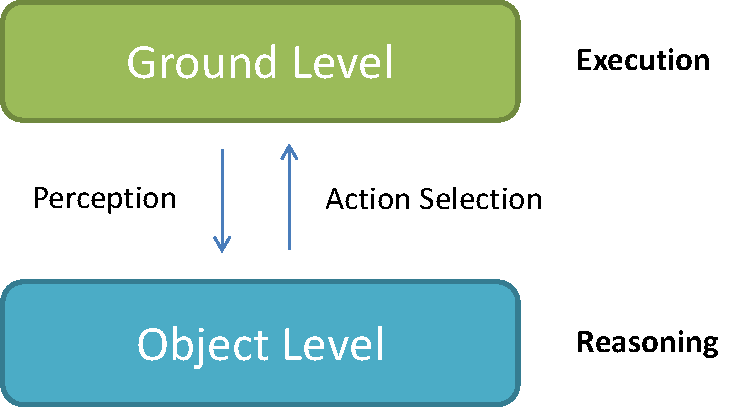
\includegraphics[width=230px]{images/reasoning}
\caption{Common cycle of perception and actions choice.}
\label{fig:reasoning}
\end{figure}

\textit{Meta-reasoning} or \textit{meta-level reasoning} is the process of explicitly reasoning about this reasoning cycle. 
It consists of both the control, and monitoring of the object-level reasoning, allowing an agent to adapt the reasoning cycle over time, as illustrated in Figure~\ref{fig:metareasoning}. 
This new cycle represents a high level reflection about its own reasoning cycle. 

\begin{figure}[ht]
\centering
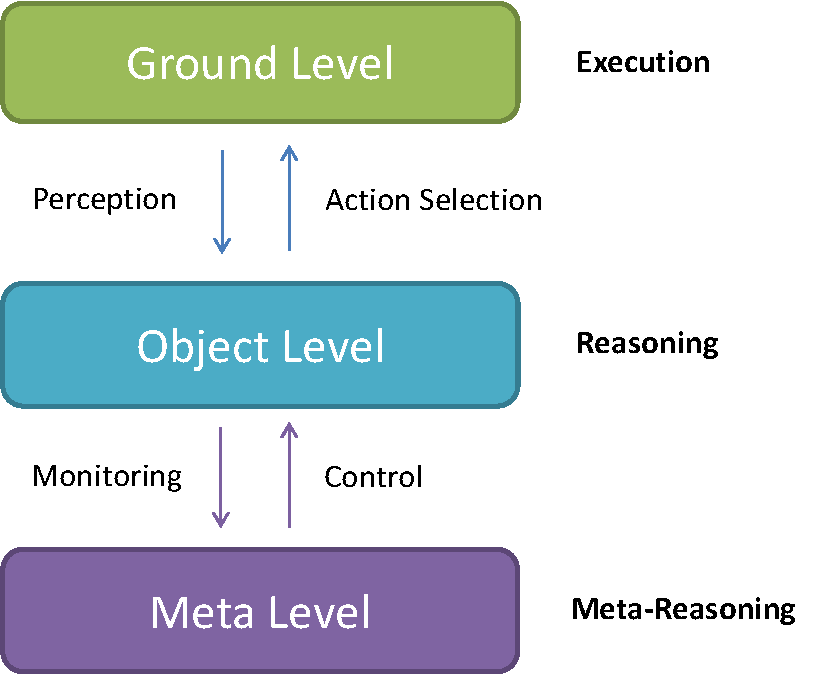
\includegraphics[width=230px]{images/metareasoning}
\caption{Adding meta-level reasoning to the common cycle of perception and choice of actions.}
\label{fig:metareasoning}
\end{figure}

When meta-level reasoning is applied to learning algorithms, this gives rise to a new term: \textit{meta-learning}~\cite{schweighofer2003meta, doya2002metalearning}.
Meta-learning represents the concept of learning to learn, and the meta-learning level is generally responsible for controlling the parameters of the learning level.
While learning at the object-level is responsible for accumulating experience about some task (e.g, take decisions in a game, medical diagnosis, fraud detection, etc.), learning at the meta-level is responsible for accumulating experience about learning algorithm itself. 
If learning at object-level is not succeeding in improving or maintaining performance, the meta-level learner takes the responsibility to adapt the object-level, in order to make it succeed.
In other words, meta-learning helps solve important problems in the application of machine learning algorithms~\cite{vilalta2004using}, especially in dynamic environments.